% move all configuration stuff into includes file so we can focus on the content
\documentclass[aspectratio=169,hyperref={pdfpagelabels=false,colorlinks=true,linkcolor=white,urlcolor=blue},t]{beamer}

%%%%%%%%%%%%%%%%%%%%%%%%%%%%%%%%%%%%%%%%%%%%%%%%%%%%%%%%%%%%%%%%%%%%%%%%%%%%%%%%%%
%%%%%%%%%%%%%%%%%%%%%%%%%%%%%%%%%%%%%%%%%%%%%%%%%%%%%%%%%%%%%%%%%%%%%%%%%%%%%%%%%%
% packages
\usepackage{pict2e}
\usepackage{epic}
\usepackage{amsmath,amsfonts,amssymb}
\usepackage{units}
\usepackage{fancybox}
\usepackage[absolute,overlay]{textpos} 
\usepackage{media9} % avi2flv: "C:\Program Files\ffmpeg\bin\ffmpeg.exe" -i TuneFreqFilterbank.avi -b 600k -s 441x324 -r 15 -acodec copy TuneFreqFilterbank.flv
\usepackage{animate}
\usepackage{gensymb}
\usepackage{multirow}
\usepackage{silence}
\usepackage[backend=bibtex,style=ieee]{biblatex}
\AtEveryCitekey{\iffootnote{\tiny}{}}
\addbibresource{references}

%%%%%%%%%%%%%%%%%%%%%%%%%%%%%%%%%%%%%%%%%%%%%%%%%%%%%%%%%%%%%%%%%%%%%%%%%%%%%%%%%%
%%%%%%%%%%%%%%%%%%%%%%%%%%%%%%%%%%%%%%%%%%%%%%%%%%%%%%%%%%%%%%%%%%%%%%%%%%%%%%%%%%
% relative paths
\graphicspath{{graph/}}


%%%%%%%%%%%%%%%%%%%%%%%%%%%%%%%%%%%%%%%%%%%%%%%%%%%%%%%%%%%%%%%%%%%%%%%%%%%%%%%%%%
%%%%%%%%%%%%%%%%%%%%%%%%%%%%%%%%%%%%%%%%%%%%%%%%%%%%%%%%%%%%%%%%%%%%%%%%%%%%%%%%%%
% units
\setlength{\unitlength}{1mm}

%%%%%%%%%%%%%%%%%%%%%%%%%%%%%%%%%%%%%%%%%%%%%%%%%%%%%%%%%%%%%%%%%%%%%%%%%%%%%%%%%%
%%%%%%%%%%%%%%%%%%%%%%%%%%%%%%%%%%%%%%%%%%%%%%%%%%%%%%%%%%%%%%%%%%%%%%%%%%%%%%%%%%
% theme & layout
\usetheme{Frankfurt}
\beamertemplatenavigationsymbolsempty
%\setbeamertemplate{frametitle}[smoothbars theme]
\setbeamertemplate{frametitle}
{
    \begin{beamercolorbox}[ht=1.8em,wd=\paperwidth]{frametitle}
        \vspace{-.1em}%
        \hspace{.2em}{\strut\insertframetitle\strut}
        
        \hspace{.2em}\small\strut\insertframesubtitle\strut
        %\hfill
        %
\includegraphics[height=.8cm,keepaspectratio]{CenterMusicTechnology-solid-2lines-white-CoAtag}
        
    \end{beamercolorbox}
    \begin{textblock*}{100mm}(11.6cm,.7cm)
        \includegraphics[height=.8cm,keepaspectratio]{logo_GTCMT_black}
    \end{textblock*}
}

% set this to ensure bulletpoints without subsections
\usepackage{remreset}
\makeatletter
\@removefromreset{subsection}{section}
\makeatother
\setcounter{subsection}{1}

%---------------------------------------------------------------------------------
% appearance
\setbeamercolor{structure}{fg=gtgold}
\setbeamercovered{transparent} %invisible
\setbeamercolor{bibliography entry author}{fg=black}
\setbeamercolor*{bibliography entry title}{fg=black}
\setbeamercolor*{bibliography entry note}{fg=black}

%\usepackage{pgfpages}
%\setbeameroption{show notes}
%\setbeameroption{show notes on second screen=right}
%---------------------------------------------------------------------------------
% fontsize
\let\Tiny=\tiny

%%%%%%%%%%%%%%%%%%%%%%%%%%%%%%%%%%%%%%%%%%%%%%%%%%%%%%%%%%%%%%%%%%%%%%%%%%%%%%%%%%
%%%%%%%%%%%%%%%%%%%%%%%%%%%%%%%%%%%%%%%%%%%%%%%%%%%%%%%%%%%%%%%%%%%%%%%%%%%%%%%%%%
% warnings
\pdfsuppresswarningpagegroup=1
\WarningFilter{biblatex}{Patching footnotes failed}
\WarningFilter{latexfont}{Font shape}
\WarningFilter{latexfont}{Some font shapes}
\WarningFilter{gensymb}{Not defining}


%%%%%%%%%%%%%%%%%%%%%%%%%%%%%%%%%%%%%%%%%%%%%%%%%%%%%%%%%%%%%%%%%%%%%%%%%%%%%%%%%%
%%%%%%%%%%%%%%%%%%%%%%%%%%%%%%%%%%%%%%%%%%%%%%%%%%%%%%%%%%%%%%%%%%%%%%%%%%%%%%%%%%
% title information
\title[]{Introduction to Audio Content Analysis}   
\author[alexander lerch]{alexander lerch} 
%\institute{~}
%\date[Alexander Lerch]{}
\titlegraphic{\vspace{-16mm}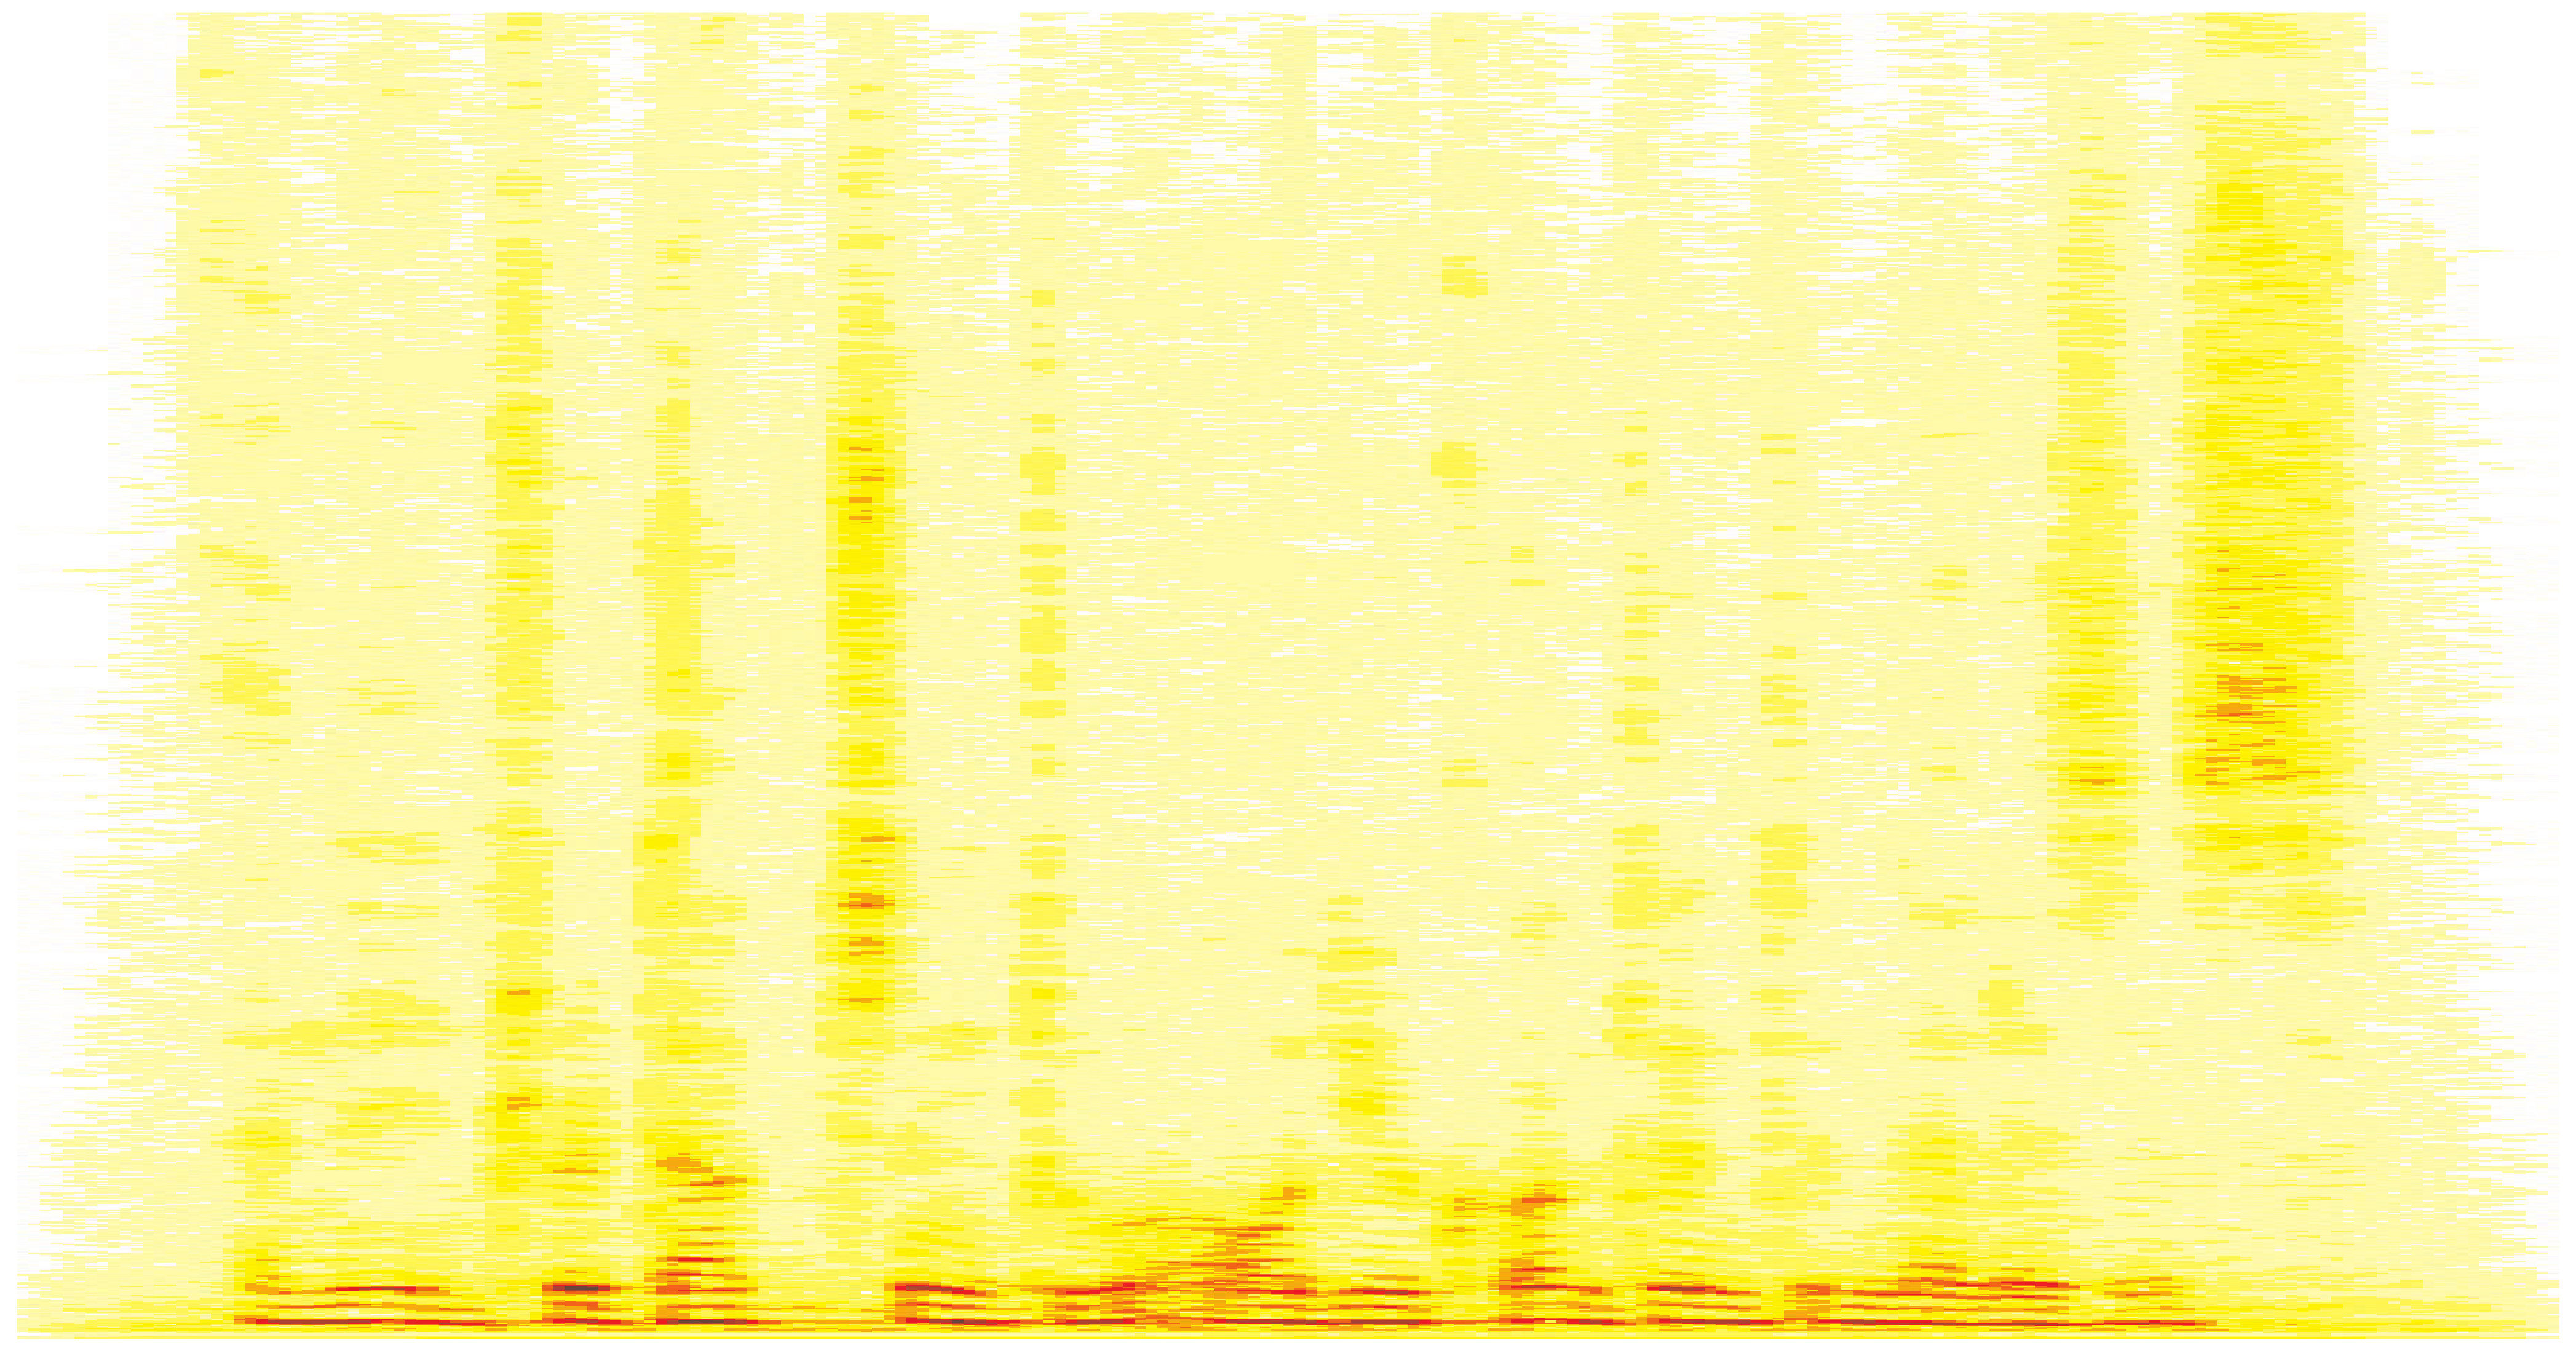
\includegraphics[width=\textwidth,height=3cm]{title}}

%%%%%%%%%%%%%%%%%%%%%%%%%%%%%%%%%%%%%%%%%%%%%%%%%%%%%%%%%%%%%%%%%%%%%%%%%%%%%%%%%%
%%%%%%%%%%%%%%%%%%%%%%%%%%%%%%%%%%%%%%%%%%%%%%%%%%%%%%%%%%%%%%%%%%%%%%%%%%%%%%%%%%
% colors
\definecolor{gtgold}{HTML}{E0AA0F} %{rgb}{0.88,0.66,1,0.06} [234, 170, 0]/256

%%%%%%%%%%%%%%%%%%%%%%%%%%%%%%%%%%%%%%%%%%%%%%%%%%%%%%%%%%%%%%%%%%%%%%%%%%%%%%%%%%
%%%%%%%%%%%%%%%%%%%%%%%%%%%%%%%%%%%%%%%%%%%%%%%%%%%%%%%%%%%%%%%%%%%%%%%%%%%%%%%%%%
% math
\DeclareMathOperator*{\argmax}{argmax}
\DeclareMathOperator*{\argmin}{argmin}
\DeclareMathOperator*{\atan}{atan}
\DeclareMathOperator*{\arcsinh}{arcsinh}
\DeclareMathOperator*{\sign}{sign}
\DeclareMathOperator*{\tcdf}{tcdf}
\DeclareMathOperator*{\si}{sinc}
\DeclareMathOperator*{\princarg}{princarg}
\DeclareMathOperator*{\arccosh}{arccosh}
\DeclareMathOperator*{\hwr}{HWR}
\DeclareMathOperator*{\flip}{flip}
\DeclareMathOperator*{\sinc}{sinc}
\DeclareMathOperator*{\floor}{floor}
\newcommand{\e}{{e}}
\newcommand{\jom}{\mathrm{j}\omega}
\newcommand{\jOm}{\mathrm{j}\Omega}
\newcommand   {\mat}[1]    		{\boldsymbol{\uppercase{#1}}}		%bold
\renewcommand {\vec}[1]    		{\boldsymbol{\lowercase{#1}}}		%bold

%%%%%%%%%%%%%%%%%%%%%%%%%%%%%%%%%%%%%%%%%%%%%%%%%%%%%%%%%%%%%%%%%%%%%%%%%%%%%%%%%%
%%%%%%%%%%%%%%%%%%%%%%%%%%%%%%%%%%%%%%%%%%%%%%%%%%%%%%%%%%%%%%%%%%%%%%%%%%%%%%%%%%
% media9
\newcommand{\includeaudio}[1]{{\includemedia[
                        addresource=audio/#1.mp3,
                        width=5mm,
                        height=5mm,
                        activate=onclick,
                        flashvars={
                            source=audio/#1.mp3  
                            &autoPlay=true
                        }]
                        {
\includegraphics[width=5mm, height=5mm]{SpeakerIcon}}
                        {APlayer.swf}}}
\newcommand{\audioautoplay}[1]{{\begin{center}\includemedia[
                            addresource=audio/#1.mp3,
                            width=.1\linewidth,
                            height=.01\linewidth,
                            activate=pageopen,
                            flashvars={
                                source=audio/#1.mp3  
                                &autoPlay=true
                            }]
                            {}
                            {APlayer.swf}\end{center}}}

\newcommand{\includevideo}[1]{{\begin{center}\includemedia[
                        addresource=video/#1.mp4,
                        width=0.8\linewidth,
                        height=0.4\linewidth,
                        activate=onclick,
                        flashvars={
                            source=video/#1.mp4  
                            &autoPlay=true
                        }]
                        {}
                        {VPlayer.swf}\end{center}}}
\newcommand{\videowithmatlab}[1]{{\begin{center}\includemedia[
                        addresource=video/animate#1.mp4,
                        width=0.8\linewidth,
                        height=0.4\linewidth,
                        activate=onclick,
                        flashvars={
                            source=video/animate#1.mp4  
                            &autoPlay=true
                        }]
                        {}
                        {VPlayer.swf}\end{center}\addreference{matlab source: matlab/animate#1.m}}}
                        

%%%%%%%%%%%%%%%%%%%%%%%%%%%%%%%%%%%%%%%%%%%%%%%%%%%%%%%%%%%%%%%%%%%%%%%%%%%%%%%%%%
%%%%%%%%%%%%%%%%%%%%%%%%%%%%%%%%%%%%%%%%%%%%%%%%%%%%%%%%%%%%%%%%%%%%%%%%%%%%%%%%%%
% other commands
\newcommand{\question}[1]{%\vspace{-4mm}
                          \setbeamercovered{invisible}
                          \begin{columns}[T]
                            \column{.8\textwidth}
                                \textbf{#1}
                            \column{.2\textwidth}
                                \vspace{-8mm}
                                \begin{flushright}
                                     
\includegraphics[scale=.5]{question_mark}
                                \end{flushright}
                                \vspace{6mm}
                          \end{columns}\pause\vspace{-12mm}}

\newcommand{\toremember}[1]{%\vspace{-4mm}
                          \begin{columns}[T]
                            \column{.8\textwidth}
                                \textbf{#1}
                            \column{.2\textwidth}
                                \vspace{-4mm}
                                \begin{flushright}
                                     
\includegraphics[scale=.5]{exclamation_mark}
                                \end{flushright}
                                \vspace{6mm}
                          \end{columns}\vspace{-6mm}}

\newcommand{\matlabexercise}[1]{%\vspace{-4mm}
                          \setbeamercovered{invisible}
                          \begin{columns}[T]
                            \column{.8\textwidth}
                                \textbf{matlab exercise}: #1
                            \column{.2\textwidth}
                                \begin{flushright}
                                     
\includegraphics[scale=.5]{logo_matlab}
                                \end{flushright}
                                %\vspace{6mm}
                          \end{columns}}

\newcommand{\addreference}[1]{  
                  
                    \begin{textblock*}{\baselineskip }(1.12\textwidth,.3\textheight) %(1.15\textwidth,.4\textheight)
                        \rotatebox{90}{\tiny {#1}}
                    \end{textblock*}}
                    
\newcommand{\figwithmatlab}[1]{
                    \begin{figure}
                        \centering
                        \includegraphics{#1}
                        %\label{fig:#1}
                    \end{figure}
                    
                    \addreference{matlab source: \href{https://github.com/alexanderlerch/ACA-Slides/blob/master/matlab/display#1.m}{matlab/display#1.m}}}
\newcommand{\figwithref}[2]{
                    \begin{figure}
                        \centering
                        \includegraphics{#1}
                        \label{fig:#1}
                    \end{figure}
                    
                    \addreference{#2}}  
                                    
\newcommand{\inserticon}[1]{

                    \begin{textblock*}{100mm}(14.5cm,7.5cm)
                        \includegraphics[height=.8cm,keepaspectratio]{#1}
                    \end{textblock*}}            

%%%%%%%%%%%%%%%%%%%%%%%%%%%%%%%%%%%%%%%%%%%%%%%%%%%%%%%%%%%%%%%%%%%%%%%%%%%%%%%%%%
%%%%%%%%%%%%%%%%%%%%%%%%%%%%%%%%%%%%%%%%%%%%%%%%%%%%%%%%%%%%%%%%%%%%%%%%%%%%%%%%%%
% counters
\newcounter{i}
\newcounter{j}
\newcounter{iXOffset}
\newcounter{iYOffset}
\newcounter{iXBlockSize}
\newcounter{iYBlockSize}
\newcounter{iYBlockSizeDiv2}
\newcounter{iDistance}



\subtitle{Module 5.2: Fundamental Frequency Detection in Monophonic Signals}

%%%%%%%%%%%%%%%%%%%%%%%%%%%%%%%%%%%%%%%%%%%%%%%%%%%%%%%%%%%%%%%%%%%%%%%%%%%%
\begin{document}
    % generate title page
	

\begin{frame}
    \titlepage
    %\vspace{-5mm}
    \begin{flushright}
        \href{http://www.gtcmt.gatech.edu}{\includegraphics[height=.8cm,keepaspectratio]{logo_GTCMT_black}}
    \end{flushright}
\end{frame}


    \section[overview]{lecture overview}
        \begin{frame}{introduction}{overview}
            \begin{block}{corresponding textbook section}
                    \href{http://ieeexplore.ieee.org/xpl/articleDetails.jsp?arnumber=6331122}{Chapter 5~---~Tonal Analysis}: pp.~91--103
            \end{block}

            \begin{itemize}
                \item   \textbf{lecture content}
                    \begin{itemize}
                        \item   established approaches to monophonic pitch tracking in
                            \begin{itemize}
                                \item   time domain
                                \item   frequency domain
                            \end{itemize}
                        \item   
                    \end{itemize}
                \bigskip
                \item<2->   \textbf{learning objectives}
                    \begin{itemize}
                        \item   define the task of monophonic pitch tracking
                        \item   summarize the principles between time-domain $f_0$-trackers and describe one detailed examples
                        \item   summarize the principles between frequency-domain $f_0$-trackers and describe one detailed examples
                    \end{itemize}
            \end{itemize}
            \inserticon{directions}
        \end{frame}

    \section[intro]{introduction}

	\begin{frame}{fundamental frequency}{introduction}
        \begin{block}{\textbf{remember}}
            Fourier series: every (quasi-)periodic sound is a combination of sinusoidals with integer frequency ratios
        \end{block}
        \begin{eqnarray*}
            x(t) 	&\approx& x(t+T_0)\nonumber\\
            x(t) &\approx& \sum\limits_{k=-\infty}^{\infty} a(k) \e^{\jom_0kt}\nonumber
        \end{eqnarray*}
        
		\begin{itemize}
			\item<2->[]	$f_0$: musically, perceptually most ``relevant'' frequency
		\end{itemize}
        \only<2->{
        \begin{figure}[t]
            \centering
            
\includegraphics[scale=.7]{pitch_harmonics}
        \end{figure}
        }
	\end{frame}
	
	%\begin{frame}{monophonic fundamental frequency detection}{pre-processing}
		%examples for pre-processing steps
		%\begin{itemize}
			%\item	\textbf{downmixing}:\\ identical fundamental frequency in all channels
			%\pause
			%\item	\textbf{low-pass filter}:\\ cut off high partials
			%\pause
			%\item	\textbf{high-pass filter}:\\ remove DC and unnecessary bass frequencies
			%\pause
			%\item	(\textbf{pre-whitening}:)\\ remove spectral envelope to receive time domain pulse train
			%\item	\ldots
		%\end{itemize}
	%\end{frame}
    
    \section[mono f0]{monophonic pitch tracking}
        \begin{frame}{pitch detection}{task definition}
            \begin{itemize}
                \item   detect the fundamental frequency $f_0$
                \item   there is only one fundamental frequency at a time
                \bigskip
                \item   related subtasks:
                    \begin{itemize}
                        \item   detect when there is no fundamental frequency
                        \item   segment into notes
                            \begin{itemize}
                                \item   start time and stop time
                                \item   average not frequency
                                \item   vibrato detection
                            \end{itemize}
                        \item   map to pitch scale
                    \end{itemize}
            \end{itemize}
        \end{frame}

	\section[time domain]{time domain methods}
	\begin{frame}{monophonic fundamental frequency detection}{zero crossing rate}
		\begin{itemize}
			\item	\textbf{number of zero crossings per block} (inaccurate)
				\begin{equation*}
					T_0(n) = \frac{2\cdot \big(i_{\mathrm{e}}(n)-i_{\mathrm{s}}(n)\big)}{f_{\mathrm{S}}\cdot\sum\limits_{i=i_{\mathrm{s}}(n)}^{i_{\mathrm{e}}(n)}{\left|\sign \left[x(i)\right]-\sign \left[x(i-1)\right]\right|}} 
				\end{equation*}
			\item<2->	\textbf{average period length}
				\begin{equation*}
					T_0(n) = \frac{2}{\mathcal{Z}-1}\sum\limits_{j=0}^{\mathcal{Z}-2}{\Delta t_\mathrm{ZC}(j)}.
				\end{equation*}
			\item<3->	\textbf{variants}:
				\begin{itemize}
					\item	create histogram with distances and choose maximum
					\item	use not (only) ZC but distance between local extrema
				\end{itemize}
		\end{itemize}
	\end{frame}
	
	\begin{frame}{monophonic fundamental frequency detection}{auto correlation function}
		\vspace{-2mm}
        \begin{itemize}
            \item find \textbf{lag of ACF maximum}
                \begin{equation*}
                    r_{xx}(\eta,n) = \sum\limits_{i=i_{\mathrm{s}}(n)}^{i_{\mathrm{e}}(n)-\eta}{x(i)\cdot x(i+\eta)}
                \end{equation*}
            \item<2->     \textbf{variants}:
                \begin{itemize}
                    \item<3->	center clipping
                            \begin{figure}
                                \centering
                                \begin{footnotesize}
	\begin{picture}(80,37)

	%%%%%%%%%%%%%%%%%%%%%%%%%%%
	% normal center clipping	
	\put(0, 21)
	{\vector(1,0){32}}
	\put(16, 5)
	{\vector(0,1){32}}
	
	\put(30, 23)
	{\text{{\shortstack[c]{$x$}}}}
	
	\put(8, 35)
	{\text{{\shortstack[c]{$\chi(x)$}}}}
	
	\put(2, 18)
	{\text{{\footnotesize{\shortstack[c]{$-c_\mathrm{L}$}}}}}
	
	\put(22, 18)
	{\text{{\footnotesize{\shortstack[c]{$+c_\mathrm{L}$}}}}}


	%%%%%%%%%%%%%%%%%%%%%%%%%%%
	% 3-level center clipping	
	\put(48, 21)
	{\vector(1,0){32}}
	\put(64, 5)
	{\vector(0,1){32}}

	\put(63.5, 13)
	{\line(1,0){1}}
	\put(63.5, 29)
	{\line(1,0){1}}
	
	\put(78, 23)
	{\text{{\shortstack[c]{$x$}}}}
	
	\put(56, 35)
	{\text{{\shortstack[c]{$\chi'(x)$}}}}
	
	\put(50, 18)
	{\text{{\footnotesize{\shortstack[c]{$-c_\mathrm{L}$}}}}}
	
	\put(70, 18)
	{\text{{\footnotesize{\shortstack[c]{$+c_\mathrm{L}$}}}}}
	
	\put(65, 13)
	{\text{{\footnotesize{\shortstack[c]{$-1$}}}}}
	
	\put(65, 29)
	{\text{{\footnotesize{\shortstack[c]{$+1$}}}}}
	
	
	% transfer functions

	\linethickness{0.5mm}	
	
	\put(8, 21)
	{\line(0,-1){8}}
	\put(24, 21)
	{\line(0,1){8}}
	\put(8, 13)
	{\line(-1,-1){8}}
	\put(24, 29)
	{\line(1,1){8}}
	\put(8, 21)
	{\line(1,0){16}}
	
	
	\put(56, 21)
	{\line(0,-1){8}}
	\put(72, 21)
	{\line(0,1){8}}
	\put(56, 13)
	{\line(-1,0){8}}
	\put(72, 29)
	{\line(1,0){8}}
	\put(56, 21)
	{\line(1,0){16}}

	\end{picture}
\end{footnotesize}

                                \label{fig:centerclipping}
                            \end{figure}
                   % \item<4->	pre-whitening: LP, spectral envelope estimation															
                \end{itemize}
        \end{itemize}
		
            
	\end{frame}
	
	\begin{frame}{monophonic fundamental frequency detection}{average magnitude difference function}
        \begin{itemize}
            \item find \textbf{lag of AMDF minimum}
                \begin{equation*}
                    \mathrm{AMDF}_{xx}(\eta,n) = \frac{1}{i_{\mathrm{e}}(n)-i_{\mathrm{s}}(n)+1}\sum\limits_{i=i_{\mathrm{s}}(n)}^{i_{\mathrm{e}}(n)-\eta}{|x(i)- x(i+\eta)|} 
                \end{equation*}
            \item<2-> \textbf{variants}:
                \begin{itemize}
                    \item	AMDF-weighted ACF
                        \begin{equation*}
                            r_{xx}'(\eta,n) = \frac{r_{xx}(\eta,n)}{\mathrm{AMDF}_{xx}(\eta,n) + 1} 
                        \end{equation*}
                \end{itemize}
        \end{itemize}
	\end{frame}
	
    \section[frequency domain]{frequency domain methods}
	\begin{frame}{monophonic fundamental frequency detection}{harmonic product spectrum 1/2}
        \vspace{-10mm}
        \begin{columns}
            \column{0.5\textwidth}
                \vspace{4mm}
                \begin{equation*}\label{eq:hps}
                    X_{\mathrm{HPS}}(k,n) = \prod\limits_{j=1}^{\mathcal{O}}{|X(j\cdot k,n)|^2}
                \end{equation*}
                
                first published in the 1960s by Noll (graph from that paper)
            \column{0.5\textwidth}
				\begin{figure}
                    \includegraphics[scale=.25]{HPS_Noll}
                \end{figure}
		\end{columns}
        \vspace{-5mm}
        \footfullcite{noll_pitch_1969}
	\end{frame}
	
	\begin{frame}{monophonic fundamental frequency detection}{harmonic product spectrum 2/2}
		\figwithmatlab{HarmonicProductSpectrum}
	\end{frame}
	
	\begin{frame}{monophonic fundamental frequency detection}{harmonic sum spectrum}
        \begin{itemize}
            \item   sum instead product sum
        \begin{equation*}\label{eq:hss}
            X_{\mathrm{HSS}}(k,n) = \sum\limits_{j=1}^{\mathcal{O}}{|X(j\cdot k,n)|^2} 
        \end{equation*}
        \bigskip

                \begin{itemize}
                    \item<1->   \textbf{advantage}
                        \begin{itemize}
                            \item   robust against missing harmonics
                        \end{itemize}
                    \item<1->   \textbf{disadvantage}
                        \begin{itemize}
                            \item   less pronounced peak
                        \end{itemize}
                \end{itemize}
        \end{itemize}
	\end{frame}
	
	\begin{frame}{monophonic fundamental frequency detection}{ACF of magnitude spectrum}
        \vspace{-3mm}
		\begin{equation*}
			r_{XX}(\eta,n) = \sum\limits_{k=-\mathcal{K}/2}^{\mathcal{K}/2-1}{|X(k,n)|\cdot |X(k+\eta,n)|}
		\end{equation*}
		\pause
		$\Rightarrow$ \textbf{detect maximum location}
        
        \vspace{-1mm}
        \only<2->{
		\figwithmatlab{AcfOfFft}
        }
	\end{frame}
	
	\begin{frame}{monophonic fundamental frequency detection}{cepstral pitch detection}
		\begin{enumerate}
			\item	compute cepstrum
			\item	detect periodicities
		\end{enumerate}
		\figwithmatlab{Cepstrum}
	\end{frame}
	
	\begin{frame}{monophonic fundamental frequency detection}{spectral maximum likelihood}
        \begin{itemize}
            \item   create \textbf{template matrix} with (smoothed) delta pulses for all possible frequencies
            
            \item<2->   compute the \textbf{cross correlation} ($lag=0$) between spectrum and all templates
            
            \item<3->   pick the result with the \textbf{highest correlation} $\Rightarrow$ frequency estimate (graph see \footfullcite{cuadra_website})
        \end{itemize}
        \only<3->{
		\begin{figure}
			\centering
				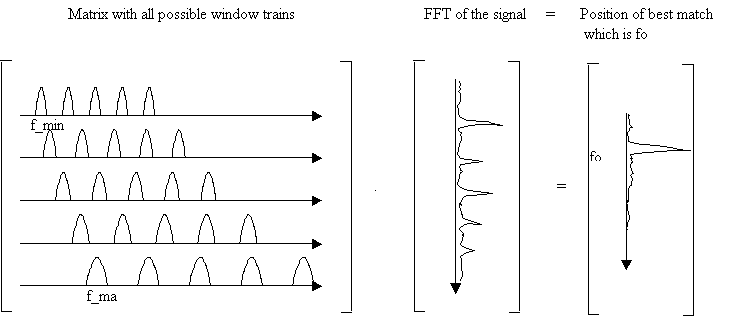
\includegraphics[scale=.4]{graph/pitch_maximumlikelihood}
		\end{figure}
        }
	\end{frame}
	
	\begin{frame}{monophonic fundamental frequency detection}{auditory-motivated pitch tracking 1/2}
		\begin{enumerate}
			\item	\textbf{filterbank} of band bass filters (e.g., mel scale)
			\item<2->	\textbf{HWR}
			\item<3->	\textbf{smoothing}
			\item<4->	within-band periodicity estimate (e.g. \textbf{ACF})
			\item<5->	\textbf{combination} of bands
		\end{enumerate}
	\end{frame}
	
	\begin{frame}{monophonic fundamental frequency detection}{auditory-motivated pitch tracking 2/2}
        \begin{columns}
        \column{.3\linewidth}
            \begin{enumerate}
                \item   filterbank output
                \bigskip
                \bigskip
                \bigskip
                \item   half wave rectification
                \bigskip
                \bigskip
                \bigskip
                \item   smoothed output
            \end{enumerate}
        \column{.7\linewidth}
            \vspace{-13mm}
            \begin{figure}%
            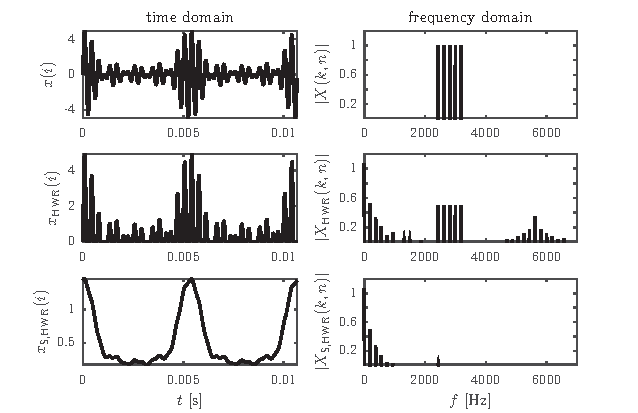
\includegraphics[width=1.1\columnwidth]{AuditoryPitchTracking}%
            \end{figure}
        \end{columns}
        \addreference{matlab source: \href{https://github.com/alexanderlerch/ACA-Slides/blob/master/matlab/displayAuditoryPitchTracking.m}{matlab/displayAuditoryPitchTracking.m}}
	\end{frame}
    
	%\begin{frame}{monophonic fundamental frequency detection}{matlab exercise}
		%\matlabexercise{monophonic pitch tracking}
        %\begin{enumerate}
            %\item   implement HPS (blocksize 2048, hopsize 512, order 5)
            %\item   implement AMDF  (blocksize 2048, hopsize 512)
            %\item   plot the pitch results (MIDI pitch) for \texttt{sax\_example.wav} from the repository
            %\item   discuss the differences in the result. what are typical errors for the implemented algorithms 
        %\end{enumerate}
	%\end{frame}
        
    \section{summary}
        \begin{frame}{summary}{lecture content}
            \begin{itemize}
                \item   \textbf{basic approach}
                    \begin{itemize}
                        \item   all approaches look for \textbf{periodicity}
                            \begin{itemize}
                                \item   waveform similarity in time domain
                                \item   equidistant harmonics/peaks in freq domain
                            \end{itemize}
                        \item   
                    \end{itemize}
                \bigskip
                \item   \textbf{state-of-the-art}
                    \begin{itemize}
                        \item   despite the age of the presented methods, tweaked versions of the presented approaches are still often considered state-of-the-art
                        \item   especially combinations of different approaches can be very successful
                    \end{itemize}
            \end{itemize}
            \inserticon{summary}
        \end{frame}
\end{document}
